% !TEX root = main.tex

\section{Lecture 4: The advection Equation (and some related jargon)}
\begin{flushright}\textbf{[by Denise Fernandez]}\end{flushright}

We have discussed the diffusion equation in Lecture~\ref{sec:lecture2}, where we considered the difference between the random molecular motion versus the motion of the centre of mass of all constituents of a fluid. Here ``advection" refers to the movement of fluid from place to place in reversible physical processes while diffusion considers irreversible exchanges and mixing processes where the matter content and thermodynamics of a fluid element are altered \citep{Griffies2019}. 

In this lecture we consider the macroscopic motion of a fluid element. The material derivative of the tracer concentration $C$ of the fluid remains constant as the element moves with the fluid (Fig. \ref{fig:trajC}), that is $C(\boldsymbol{x},t)= C[\boldsymbol{x}(0)]$ and 

\begin{equation}
    \frac{\mathrm{D}C}{\mathrm{D}t}= \frac{\partial C}{\partial t} + \boldsymbol{v} \cdot \boldsymbol{\nabla} C = 0.
    \label{Eq:adv1}
\end{equation}

\begin{figure}[h]
\centering
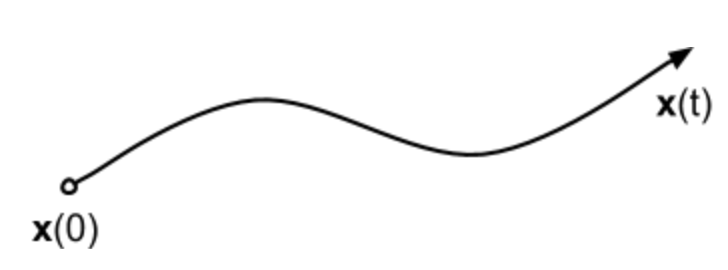
\includegraphics[width=0.3\textwidth]{figures/Lecture4_fig1.png}
\caption{Trajectory of the tracer concentration $C$ with no diffusion, just transport of the particle.}
\label{fig:trajC}
\end{figure}

Here we use the chain rule and the constancy of the tracer concentration to show that advection of the transport concentration is reversible,

\begin{equation}
    \frac{DC}{Dt}^{\alpha} = C ^{\alpha -1} \frac{DC}{Dt} = 0.
    \label{Eq:adv2}
\end{equation}

where $\alpha$ is an arbitrary number. 
\subsection{Mass transport from the mean, eddy and residual mean}

The density $\rho$ is an example of such a tracer and evolves according to:
\begin{equation}
    \frac{\partial \rho}{\partial t}= -\boldsymbol{\nabla} \cdot (\boldsymbol{v}\rho).
    \label{Eq:tend1}
\end{equation}

The mass density time tendency (i.e., $\partial \rho/\partial t$) remains unchanged if the advective mass flux $\rho \boldsymbol{v}$ is modified by the addition of the eddy-induced mass flux of the form $\rho\boldsymbol{v}^* = \boldsymbol{\nabla}\times(\rho\boldsymbol{\Psi})$ (where $\boldsymbol{\Psi}$ is a vector streamfunction),
\begin{align}
    \boldsymbol{v} \rho \rightarrow \boldsymbol{v}^\dagger \rho &\equiv (\boldsymbol{v} + \boldsymbol{v}^*) \rho \\
    & = \rho \boldsymbol{v} + \rho \boldsymbol{v}^*,\\
    & = \rho \boldsymbol{v} + \boldsymbol{\nabla}\times(\rho\boldsymbol{\Psi}).
        \label{Eq:add_massflx}
\end{align}

The additional mass flux $\boldsymbol{\nabla} \times (\rho \boldsymbol{\Psi}$) in Eq. \eqref{Eq:add_massflx} does not lead to accumulation of mass since its divergence is zero. This is known as ``Gauge Invariance" symmetry resulting from the decomposition of the mass flux into a mean and a non-divergent fluctuation \citep{Griffies2019}. 


The terminology is the following: %I'd like to add subequations..
\begin{subequations} %Here's how you add subequations. Awesome, thanks!
\begin{align}
    \boldsymbol{v} &= \text{Eulerian mean velocity}, \\
    \rho \boldsymbol{v} &= \text{Eulerian mean mass flux (per unit volume)}, \\
    \boldsymbol{v}^* &= \text{Eddy-induced velocity}, \\
    \rho \boldsymbol{v}^* &= \boldsymbol{\nabla} \times (\rho \boldsymbol{\Psi}) = \text{Eddy-induced mass flux}, \label{Eq:eddy_mass_flx}\\
    \boldsymbol{v}^\dagger &= \boldsymbol{v}+\boldsymbol{v}^* = \text{Residual mean velocity \space (i.e. winds$+$rotation due to eddies)}, \\
    \rho \boldsymbol{v}^\dagger &= \text{Residual mean mass flux}. 
 \end{align} 
 \end{subequations}
 
Now we turn into the tracer advection equation to derive the eddy Skew flux. 

Consider the transport concentration is determined by the residual velocity (remember: the ``eddy contribution often compensates for the mean, with sum of the mean and eddy representing a residual" \citep{Griffies2019}),
 
 \begin{equation}
     \frac{\partial (\rho C)}{\partial t} + \boldsymbol{\nabla} \cdot (\rho \boldsymbol{v}^\dagger C) = 0.
     \label{Eq:TAEq}
 \end{equation}
 
 Using Eq. \eqref{Eq:eddy_mass_flx} for the eddy-induced mass flux and the tracer advection equation with the advective transport determined by the residual mean velocity (Eq.~\eqref{Eq:TAEq}) we can write 
 \begin{align}
      \rho \boldsymbol{v}^\dagger C &= C(\rho \boldsymbol{v} + \rho \boldsymbol{v}^*) \nonumber\\
    																& = C\rho \boldsymbol{v} + C \boldsymbol{\nabla} \times (\rho \boldsymbol{\Psi}) \nonumber\\
    																&= C\rho \boldsymbol{v} + \boldsymbol{\nabla} \times (C \rho \boldsymbol{\Psi}) - \boldsymbol{\nabla} C \times \boldsymbol{\Psi} \rho.
 \end{align}	
 (Above, to go from the second to the third line we just used Leibniz rule for derivatives of products.)

 What matters for the evolution of $\rho C$ is the divergence of the tracer flux
  \begin{equation}
      \boldsymbol{\nabla} \cdot (\rho \boldsymbol{v}^\dagger C) = \boldsymbol{\nabla} \cdot (C\rho \boldsymbol{v}) - \boldsymbol{\nabla} \cdot (\boldsymbol{\nabla} C \times \rho \boldsymbol{\Psi}),
  \end{equation}
  or after bringing the $\boldsymbol{\nabla} \cdot (C\rho \boldsymbol{v})$ on the right-hand side:
  \begin{equation}
      \boldsymbol{\nabla} \cdot (\rho C \boldsymbol{v}^*) =  \boldsymbol{\nabla} \cdot (\underbrace{-\boldsymbol{\nabla} C \times \rho \boldsymbol{\Psi}}_{\text{eddy skew flux}}). \label{eq4.10}
  \end{equation}

Equation~\eqref{eq4.10} implies that 
\begin{equation}
      \substack{\text{\normalsize\textbf{Divergence of}}\\\text{\normalsize\textbf{the eddy advection flux}}} =  
			\substack{\text{\normalsize\textbf{Divergence of}}\\\text{\normalsize\textbf{the eddy skew flux}}}
\end{equation}
 and because the tracer flux does not cross iso-surfaces, that is, $\boldsymbol{\nabla} C \cdot (-\boldsymbol{\nabla} C \times \rho \boldsymbol{\Psi}) = 0$, the flux is \textbf{skew} and oriented parallel to the iso-surfaces of tracer concentration (see figure~\ref{fig:skewF}).


\begin{figure}[h]
\centering
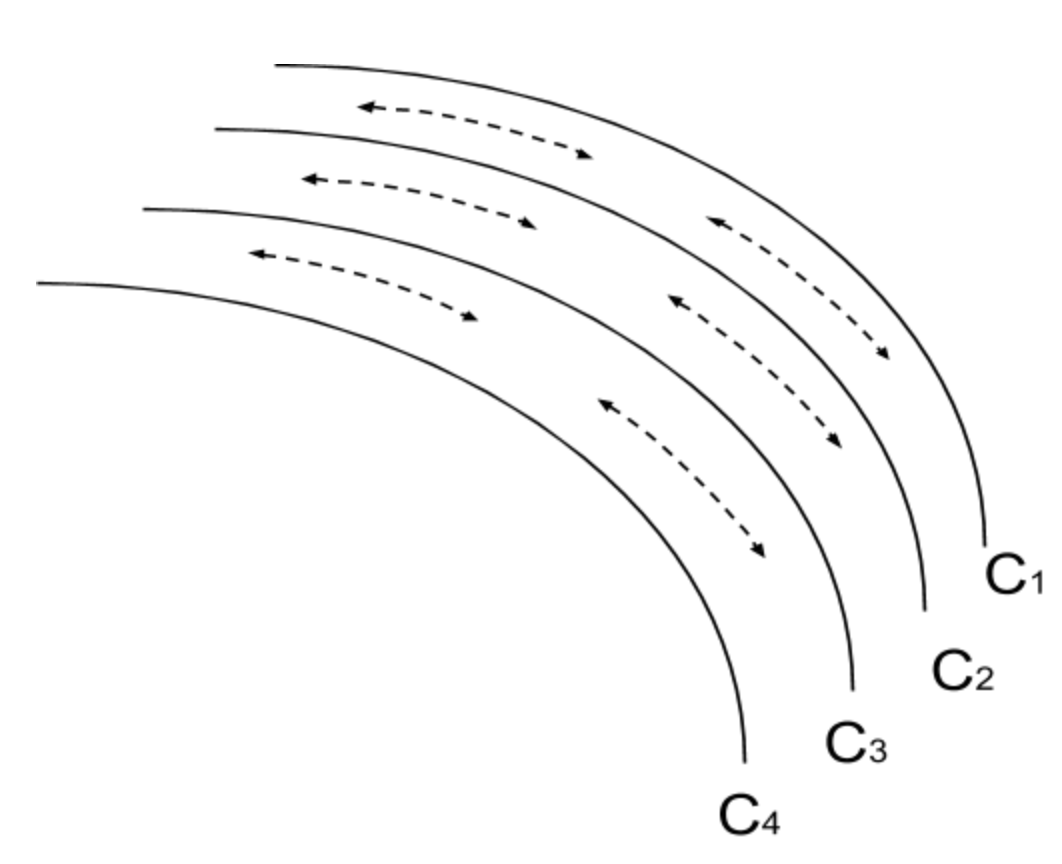
\includegraphics[width=0.3\textwidth]{figures/Lecture4_fig2.png}
\caption{Schematic of the skew fluxes (dashed arrows) for a tracer concentration $C$ parallel to iso-lines of constant $C$ (solid curves).}
\label{fig:skewF}
\end{figure}
 
 \subsection{Skew diffusion}
 {\color{red}[Navid: Andy/Stephen, this sections seems a bit out-of-context here. How should we improve it? Perhaps we should postpone it until the GM lecture?]}

 In tensor notation the advection of the Eddy Skew flux $J^{\textrm{skew}}_m = \big[ -\boldsymbol{\nabla} C \times \rho \boldsymbol{\Psi}\big]_m$ is          
\begin{align}
    J^{\textrm{skew}} _m &= \left( \epsilon_{mnp} \frac{\partial C}{\partial x^n}\right)\rho \Psi_p \\
    & = A_{mn} \frac{\partial C}{\partial x^n}
\end{align}
%ideally use \mathbb
where
\begin{equation}
A_{mn} \equiv \epsilon_{mnp} \Psi_p = \begin{pmatrix}
                                    0 & \Psi_3 & -\Psi_2\\
                                    -\Psi_3 & 0 & \Psi_1\\
                                    \Psi_2 & -\Psi_1 & 0
                                \end{pmatrix},
\end{equation}
is the \textbf{Skew diffusion tensor} and $\epsilon_{mnp}$ the Levi-Civita tensor. (For details and definition of $\epsilon_{mnp}$ refer to Lecture~\ref{sec:tensors}.)